\section{Testing}
\subsection{Testing JUnit}
I test sono stati fatti sul back-end, in particolare abbiamo scelto due metodi da fare back box (hideNotification e changePassword) e due white box (createOrder e deleteDish).
Per fare ciò sono è stato utilizzato il framework \textbf{JUnit} e \textbf{Mockito}:
\begin{itemize}
  \item \textbf{JUnit -} è un framework che permette di testare unitariamente applicazioni Java.
  \item \textbf{Mockito -} è un framework Java che permette di simulare oggetti, usato in questo caso per simulare oggetti da passare ai metodi testati.
\end{itemize}
\subsubsection{Black box testing}
\paragraph{changePassword} vista la mancanza di un recupera password, infatti se si dimentica la password l'unico che può resettarla è un amministratore, è stato scelto in quanto metodo fondamentale. Era necessario che questo metodo non fallisse.
\begin{lstlisting}[language=java]
  public EmployeeResponseDTO changePassword(String password, String email)
\end{lstlisting}
Per testare questo metodo, sono state analizzate le classi d'equivalenza, in questo caso avendo due \textbf{String} come valore non valido si aveva solo \textbf{null} mentre gli altri sono tutti validi.
Qui sotto riportiamo una tabella (cosi per tutti i metodi) che contiene i valori vali e quelli non validi, sono tutti identificati da una lettera (indica il parametro) e un numero (valido o meno).
\begin{table}[H]
  \centering
  \begin{tabular}{|p{2cm}|p{3cm}|p{2cm}|p{2cm}|p{2cm}|}
    \hline
    \rowcolor{green!10}
    \textbf{Nome parametro} & \textbf{Denominazione parametro} & \textbf{Tipo parametro} & \textbf{Esempio parametro} & \textbf{Validità parametro} \\
    \hline
    \rowcolor{black!10}
    password                & $A1$                             & String                  & null                       & non valido                  \\
    password                & $A2$                             & String                  & "stringa"                  & valido                      \\
    \hline
    \rowcolor{black!10}
    email                   & $B1$                             & String                  & null                       & non valido                  \\
    email                   & $B2$                             & String                  & "stringa"                  & valido                      \\
    \hline
  \end{tabular}
\end{table}
Adesso che abbiamo visto il dominio dei parametri, passiamo al testing. Questo metodo è stato testato tramite metodologia \textbf{SECT} (Strong Equivalence Class Testing), sono quindi state esplicitate tutte le classi d'equivalenza, arrivando cos' a 4 metodi di testing.
\begin{lstlisting}[language=java]
@ExtendWith(MockitoExtension.class)
@ExtendWith(SpringExtension.class)
public class ChangePasswordBBT {
    @InjectMocks
    private EmployeeServiceImpl employeeServiceImpl;
    @Mock
    private EmployeeService employeeService;
    @Mock
    private EmployeeRepository employeeRepository;

    @Test
    public void changePassword_A1_B1(){
        assertThrows(UsernameNotFoundException.class, () ->{
        employeeServiceImpl.changePassword(null, null);
    });
    }

    @Test
    public void changePassword_A1_B2(){
        String email = "paolo";
        assertThrows(UsernameNotFoundException.class, () ->{
            employeeServiceImpl.changePassword(null, email);
        });
    }
    @Test
    public void changePassword_A2_B1(){
        String password= "null";
        assertThrows(UsernameNotFoundException.class, () ->{
            employeeServiceImpl.changePassword(password, null);
        });
    }
    @Test
    public void changePassword_A2_B2(){
        Employee employee = new Employee("paolo",
                "cammardella",
                "prova",
                Employee.Role.ADDETTO_CUCINA,
                false);

        when(employeeRepository.findByEmail(employee.getEmail())).thenReturn(employee);
        EmployeeResponseDTO employeeChangePasswd = employeeServiceImpl.changePassword(employee.getPassword(), employee.getEmail());
        assertEquals(true, employeeChangePasswd.getRequestSuccess());
    }
}
\end{lstlisting}
\paragraph{hideNotification} abbiamo deciso di testare questo metodo, in quanto è fondamentale per la corretta gestione dell'attività di ristorazione. Basti pensare che le notifiche sono l'unica cosa comune a tutti i ruoli, se quindi dovesse esserci un problema ne risentirebbe il maggior numero di utenti.
\begin{lstlisting}[language=java]
  public NotificationResponseDTO hideNotification(Notification hiddenNotification, Employee creatorEmployee)
\end{lstlisting}
Come per il precedente metodo, sono state analizzate le classi d'equivalenza, in questo caso però non è stato cosi semplice, infatti i parametri passati a questo metodo sono più complessi per quanto riguarda la loro composizione.
Il valore non valido per i campi di entrambi gli oggetti, è \textbf{null}, quello valido invece è una stringa generica.
\begin{table}[H]
  \centering
  \begin{tabular}{|p{2cm}|p{3cm}|p{2cm}|p{2cm}|p{2cm}|}
    \hline
    \multicolumn{5}{|c|}{Employee creatoreEmployee}\\
    \hline
    \rowcolor{green!10}
    \textbf{Nome parametro} & \textbf{Denominazione parametro} & \textbf{Tipo parametro} & \textbf{Esempio parametro} & \textbf{Validità parametro} \\
    \hline
    \rowcolor{black!10}
    name                    & $A1$                             & String                  & null                       & non valido                  \\
    name                    & $A2$                             & String                  & "stringa"                  & valido                      \\
    \hline
  \end{tabular}
\end{table}

\begin{table}[H]
    \centering
    \begin{tabular}{|p{2cm}|p{3cm}|p{2cm}|p{2cm}|p{2cm}|}
      \hline
      \multicolumn{5}{|c|}{Notification hiddenNotification}\\
      \hline
      \rowcolor{green!10}
      \textbf{Nome parametro} & \textbf{Denominazione parametro} & \textbf{Tipo parametro} & \textbf{Esempio parametro} & \textbf{Validità parametro} \\
      \hline
      \rowcolor{black!10}
      title                   & $B1$                             & String                  & null                       & non valido                  \\
      title                   & $B2$                             & String                  & "stringa"                  & valido                      \\
      \hline
      \rowcolor{black!10}
      text                    & $C1$                             & String                  & null                       & non valido                  \\
      text                    & $C2$                             & String                  & "stringa"                  & valido                      \\
      \hline
      \rowcolor{black!10}
      date                    & $D1$                             & String                  & null                       & non valido                  \\
      date                    & $D2$                             & String                  & "stringa"                  & valido                      \\
      \hline
      \rowcolor{black!10}
      creatoreEmail           & $E1$                             & String                  & null                       & non valido                  \\
      creatorEmail            & $E2$                             & String                  & "stringa"                  & valido                      \\
      \hline
    \end{tabular}
  \end{table}
  
\newpage
\begin{lstlisting}[language=java]
@ExtendWith(MockitoExtension.class)
@ExtendWith(SpringExtension.class)
public class HideNotificationBBT {
    @InjectMocks
    private NotificationServiceImpl notificationServiceImpl;
    @Mock
    private NotificationService notificationService;
    @Mock
    private NotificationRepository notificationRepository;
    @Mock
    private EmployeeRepository employeeRepository;
    @Mock
    private EmployeeServiceImpl employeeServiceImpl;
    @Mock
    private EmployeeService employeeService;

    Employee employee;
    Notification notification;

    @BeforeEach
    public void init() {
        employee = new Employee();
        employee.setNotifications(new ArrayList<>());
        employee.setName("Paolo");
        employee.setEmail("paolo@cammardella.it");
        employee.setPassword("ciao");
        employee.setRole(Employee.Role.ADDETTO_CUCINA);
        employee.setFirstLogin(false);
        employee.setRestaurantTables(new ArrayList<>());
        employee.setCategories(new ArrayList<>());


        notification = new Notification("notifica", "testo notifica", "12/03/1999", "paolo@cammardella.it");
        notification.setEmployees(new ArrayList<>());
        employee.getNotifications().add(notification);
        notification.getEmployees().add(employee);
        when(employeeService.findEmployeeByEmail(employee.getEmail())).thenReturn(employee);
        when(notificationRepository.findByTitleAndTextAndCreatorEmailAndDate(notification.getTitle(), notification.getText(), notification.getCreatorEmail(), notification.getDate())).thenReturn(notification);
    }


    @Test
    public void testHideNotificationA1_B1_C1_D1_E1() {
        employee.setName(null);
        notification.setTitle(null);
        notification.setText(null);
        notification.setDate(null);
        notification.setCreatorEmail(null);

        assertThrows(RuntimeException.class, () -> {
            notificationServiceImpl.hideNotification(notification, employee);
        });
    }

    @Test
    public void testHideNotificationA1_B1_C1_D1_E2() {
        employee.setName(null);
        notification.setTitle(null);
        notification.setText(null);
        notification.setDate(null);

        assertThrows(RuntimeException.class, () -> {
            notificationServiceImpl.hideNotification(notification, employee);
        });
    }

    @Test
    public void testHideNotificationA1_B1_C1_D2_E1() {
        employee.setName(null);
        notification.setTitle(null);
        notification.setText(null);
        notification.setCreatorEmail(null);

        assertThrows(RuntimeException.class, () -> {
            notificationServiceImpl.hideNotification(notification, employee);
        });
    }

    @Test
    public void testHideNotificationA1_B1_C1_D2_E2() {
        employee.setName(null);
        notification.setTitle(null);
        notification.setText(null);

        assertThrows(RuntimeException.class, () -> {
            notificationServiceImpl.hideNotification(notification, employee);
        });
    }

    @Test
    public void testHideNotificationA1_B1_C2_D1_E1() {
        employee.setName(null);
        notification.setTitle(null);
        notification.setDate(null);
        notification.setCreatorEmail(null);

        assertThrows(RuntimeException.class, () -> {
            notificationServiceImpl.hideNotification(notification, employee);
        });
    }

    @Test
    public void testHideNotificationA1_B1_C2_D1_E2() {
        employee.setName(null);
        notification.setTitle(null);
        notification.setDate(null);

        assertThrows(RuntimeException.class, () -> {
            notificationServiceImpl.hideNotification(notification, employee);
        });
    }

    @Test
    public void testHideNotificationA1_B1_C2_D2_E1() {
        employee.setName(null);
        notification.setTitle(null);
        notification.setCreatorEmail(null);

        assertThrows(RuntimeException.class, () -> {
            notificationServiceImpl.hideNotification(notification, employee);
        });
    }

    @Test
    public void testHideNotificationA1_B1_C2_D2_E2() {
        employee.setName(null);
        notification.setTitle(null);

        assertThrows(RuntimeException.class, () -> {
            notificationServiceImpl.hideNotification(notification, employee);
        });
    }

    @Test
    public void testHideNotificationA1_B2_C1_D1_E1() {
        employee.setName(null);
        notification.setText(null);
        notification.setDate(null);
        notification.setCreatorEmail(null);

        assertThrows(RuntimeException.class, () -> {
            notificationServiceImpl.hideNotification(notification, employee);
        });
    }

    @Test
    public void testHideNotificationA1_B2_C1_D1_E2() {
        employee.setName(null);
        notification.setText(null);
        notification.setDate(null);

        assertThrows(RuntimeException.class, () -> {
            notificationServiceImpl.hideNotification(notification, employee);
        });
    }

    @Test
    public void testHideNotificationA1_B2_C1_D2_E1() {
        employee.setName(null);
        notification.setText(null);
        notification.setCreatorEmail(null);

        assertThrows(RuntimeException.class, () -> {
            notificationServiceImpl.hideNotification(notification, employee);
        });
    }

    @Test
    public void testHideNotificationA1_B2_C1_D2_E2() {
        employee.setName(null);
        notification.setText(null);

        assertThrows(RuntimeException.class, () -> {
            notificationServiceImpl.hideNotification(notification, employee);
        });
    }

    @Test
    public void testHideNotificationA1_B2_C2_D1_E1() {
        employee.setName(null);
        notification.setDate(null);
        notification.setCreatorEmail(null);

        assertThrows(RuntimeException.class, () -> {
            notificationServiceImpl.hideNotification(notification, employee);
        });
    }

    @Test
    public void testHideNotificationA1_B2_C2_D1_E2() {
        employee.setName(null);
        notification.setText(null);
        notification.setDate(null);

        assertThrows(RuntimeException.class, () -> {
            notificationServiceImpl.hideNotification(notification, employee);
        });
    }

    @Test
    public void testHideNotificationA1_B2_C2_D2_E1() {
        employee.setName(null);
        notification.setCreatorEmail(null);

        assertThrows(RuntimeException.class, () -> {
            notificationServiceImpl.hideNotification(notification, employee);
        });
    }

    @Test
    public void testHideNotificationA1_B2_C2_D2_E2() {
        employee.setName(null);

        assertThrows(RuntimeException.class, () -> {
            notificationServiceImpl.hideNotification(notification, employee);
        });
    }

    @Test
    public void testHideNotificationA2_B1_C1_D1_E1() {
        notification.setTitle(null);
        notification.setText(null);
        notification.setDate(null);
        notification.setCreatorEmail(null);
        employee.getNotifications().add(notification);
        assertThrows(RuntimeException.class, () -> {
            notificationServiceImpl.hideNotification(notification, employee);
        });
    }

    @Test
    public void testHideNotificationA2_B1_C1_D1_E2() {
        notification.setTitle(null);
        notification.setText(null);
        notification.setDate(null);

        assertThrows(RuntimeException.class, () -> {
            notificationServiceImpl.hideNotification(notification, employee);
        });
    }

    @Test
    public void testHideNotificationA2_B1_C1_D2_E1() {
        notification.setTitle(null);
        notification.setText(null);
        notification.setCreatorEmail(null);
        assertThrows(RuntimeException.class, () -> {
            notificationServiceImpl.hideNotification(notification, employee);
        });
    }

    @Test
    public void testHideNotificationA2_B1_C1_D2_E2() {
        notification.setTitle(null);
        notification.setText(null);
        assertThrows(RuntimeException.class, () -> {
            notificationServiceImpl.hideNotification(notification, employee);
        });
    }

    @Test
    public void testHideNotificationA2_B1_C2_D1_E1() {
        notification.setTitle(null);
        notification.setDate(null);
        notification.setCreatorEmail(null);
        assertThrows(RuntimeException.class, () -> {
            notificationServiceImpl.hideNotification(notification, employee);
        });
    }

    @Test
    public void testHideNotificationA2_B1_C2_D1_E2() {
        notification.setTitle(null);
        notification.setDate(null);
        assertThrows(RuntimeException.class, () -> {
            notificationServiceImpl.hideNotification(notification, employee);
        });
    }

    @Test
    public void testHideNotificationA2_B1_C2_D2_E1() {
        notification.setTitle(null);
        notification.setCreatorEmail(null);
        assertThrows(RuntimeException.class, () -> {
            notificationServiceImpl.hideNotification(notification, employee);
        });
    }

    @Test
    public void testHideNotificationA2_B1_C2_D2_E2() {
        notification.setTitle(null);
        assertThrows(RuntimeException.class, () -> {
            notificationServiceImpl.hideNotification(notification, employee);
        });
    }

    @Test
    public void testHideNotificationA2_B2_C1_D1_E1() {
        notification.setText(null);
        notification.setDate(null);
        notification.setCreatorEmail(null);
        assertThrows(RuntimeException.class, () -> {
            notificationServiceImpl.hideNotification(notification, employee);
        });
    }

    @Test
    public void testHideNotificationA2_B2_C1_D1_E2() {
        notification.setText(null);
        notification.setDate(null);
        assertThrows(RuntimeException.class, () -> {
            notificationServiceImpl.hideNotification(notification, employee);
        });
    }

    @Test
    public void testHideNotificationA2_B2_C1_D2_E1() {
        notification.setText(null);
        notification.setCreatorEmail(null);
        assertThrows(RuntimeException.class, () -> {
            notificationServiceImpl.hideNotification(notification, employee);
        });
    }

    @Test
    public void testHideNotificationA2_B2_C1_D2_E2() {
        notification.setText(null);
        assertThrows(RuntimeException.class, () -> {
            notificationServiceImpl.hideNotification(notification, employee);
        });
    }

    @Test
    public void testHideNotificationA2_B2_C2_D1_E1() {
        notification.setDate(null);
        notification.setCreatorEmail(null);
        assertThrows(RuntimeException.class, () -> {
            notificationServiceImpl.hideNotification(notification, employee);
        });
    }

    @Test
    public void testHideNotificationA2_B2_C2_D1_E2() {
        notification.setText(null);
        notification.setDate(null);
        assertThrows(RuntimeException.class, () -> {
            notificationServiceImpl.hideNotification(notification, employee);
        });
    }

    @Test
    public void testHideNotificationA2_B2_C2_D2_E1() {
        notification.setCreatorEmail(null);
        assertThrows(RuntimeException.class, () -> {
            notificationServiceImpl.hideNotification(notification, employee);
        });
    }

    @Test
    public void testHideNotificationA2_B2_C2_D2_E2() {
        NotificationResponseDTO response = notificationServiceImpl.hideNotification(notification, employee);
        assertEquals(true, response.getIsSuccesful());
    }
}
\end{lstlisting}
\subsection{White box testing}
Per il testing \textit{white box} sono stati scelti due metodi più semplici da testare, fondamentale si ma meno importanti dei due fatti tramite \textit{black box testing}. Questo perché i metodi che vedremo di seguito devono essere si affidabili, ma un errore nell'esecuzione di uno di questi due metodi, sarà meno impattante sull'esperienza dell'utente.
\paragraph{createOrder} il metodo per la creazione di un ordinazione permette ad un "addetto alla sala" di aggiungere ordinazioni ad un tavolo. Di seguito viene riportato il metodo per intero:
\begin{lstlisting}[language=java]
    @Override
    public RestaurantTableDTO createOrder(RestaurantTable restaurantTable, Dish dish) {
        if (restaurantTable != null && dish != null) {
            Dish newOrderDish = dishRepository.findByName(dish.getName());
            newOrderDish.getRestaurantTables().add(restaurantTableService.findById(restaurantTable.getId()));
            dishRepository.save(newOrderDish);
            restaurantTable.getDishes().add(newOrderDish);
            return new RestaurantTableDTO(restaurantTable,
                    true, "Piatto: " + dish.getName() + " aggiunto al tavolo: " + restaurantTable.getId().toString());
        }
        return new RestaurantTableDTO(restaurantTable,
                false, "Piatto o tavolo non valido");
    }
\end{lstlisting}
Osservando questo metodo, possiamo ricavare il \textit{grafo del flusso di controllo}, che ci permetterà di seguito di testare il metodo nel miglior modo possibile:
\begin{figure}[H]
    \centering
    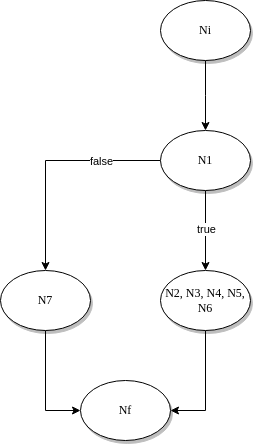
\includegraphics[scale=0.8]{img/whiteBox/createOrder.png}
    \caption{Grafo del flusso di controllo per createOrder}
\end{figure}
Osservando questo grafo, possiamo ricavare due metodi di testing in modo da ottenere un cosiddetto "\textbf{branch coverage}", ovvero facciamo in modo che ogni caso sia coperto da test:
\begin{itemize}
    \item testCreateOrder1()
    \item testCreateOrder2()
\end{itemize}
\begin{lstlisting}[language=java]
@ExtendWith(MockitoExtension.class)
@ExtendWith(SpringExtension.class)
public class CreateOrderWBT {

    @InjectMocks
    private DishServiceImpl dishServiceImpl;

    @Mock
    private DishService dishService;
    @Mock
    private DishRepository dishRepository;
    @Mock
    private RestaurantTableService restaurantTableService;

    @Test
    public void testCreateOrder1() {
        RestaurantTable restaurantTable = new RestaurantTable();
        restaurantTable.setId(1);

        Dish dish = new Dish();
        dish.setId(2);
        dish.setName("Pasta");
        dish.setCategory(new Category(1, "PRIMI", new ArrayList<Dish>()));

        when(dishRepository.findByName("Pasta")).thenReturn(dish);
        when(restaurantTableService.findById(1)).thenReturn(restaurantTable);

        RestaurantTableDTO response = dishServiceImpl.createOrder(restaurantTable, dish);
        assertEquals(restaurantTable, response.getRestaurantTable());
        assertEquals(true, response.getIsSuccessful());
        assertEquals("Piatto: Pasta aggiunto al tavolo: 1", response.getRequestInfo());
    }

    @Test
    public void testCreateOrder2() {
        RestaurantTableDTO response = dishServiceImpl.createOrder(null, null);
        assertEquals(null, response.getRestaurantTable());
        assertEquals(false, response.getIsSuccessful());
        assertEquals("Piatto o tavolo non valido", response.getRequestInfo());

    }
}

\end{lstlisting}
\paragraph{deleteDish} il metodo per l'eliminazione di un piatto, permette ad un amministratore/supervisore di eliminare un piatto dal menù. Abbiamo deciso di testare questo metodo tramite \textit{white box testing} in quanto, si fondamentale, ma un errore in questo metodo, può essere ovviato mandando una notifica con i piatti non disponibili. Ciò non vuol dire che il metodo può non funzionare. Di seguito è riportato il metodo per intero:
\begin{lstlisting}[language=java]
    @Override
    @Transactional
    public MenuResponseDTO deleteDish(String dishName, Category category) {
        if (dishRepository.existsByName(dishName)) {
            Dish dish = dishRepository.findByName(dishName);
            categoryService.printCategoryByName(category.getName()).getCategoryDishDTO().getCategory().getDishes().remove(dish);
            dishRepository.deleteByName(dishName);
            log.info("Piatto eliminato con successo: {}", dish);
            return new MenuResponseDTO(null, "Piatto eliminato con successo", true);
        }
        log.info("Piatto non trovato!");
        return new MenuResponseDTO(new CategoryDishDTO(categoryService.printCategoryByName(category.getName()).getCategoryDishDTO().getDishes(), category), "Piatto inesistente", false);
    }
\end{lstlisting}
Da questo metodo, come fatto per il precedente, possiamo ricare un grafo del flusso di controllo:
\begin{figure}[H]
    \centering
    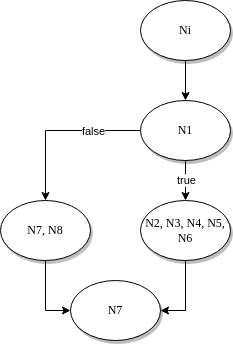
\includegraphics[scale=0.8]{img/whiteBox/deleteDish.png}
    \caption{Grafo del flusso di controllo per deleteDish}
\end{figure}
Come fatto per il precedente metodo, individuiamo i metodi che ci permettono di ottenere il branch coverage:
\begin{itemize}
    \item testDeleteDish1()
    \item testDeleteDish2()
\end{itemize}
Di seguito vengono riportati i metodi di testing.
\begin{lstlisting}[language=java]
@ExtendWith(MockitoExtension.class)
@ExtendWith(SpringExtension.class)
public class DeleteDishWBT {
    @InjectMocks
    private DishServiceImpl dishServiceImpl;
    @Mock
    private DishService dishService;
    @Mock
    private DishRepository dishRepository;

    @Mock
    private CategoryRepository categoryRepository;
    @Mock
    private CategoryService categoryService;

    @Test
    public void testDeleteDish1(){
        String dishName = "pollo";

        Category category = new Category();
        category.setName("Primi");
        category.setDishes(new ArrayList<>());

        Dish dish = new Dish();
        dish.setId(2);
        dish.setName(dishName);
        dish.setCategory(category);

        when(dishRepository.existsByName(dishName)).thenReturn(true);
        when(dishRepository.findByName(dishName)).thenReturn(dish);
        when(categoryService.printCategoryByName(category.getName())).thenReturn(new MenuResponseDTO(new CategoryDishDTO(category.getDishes(), category), "Piatto eliminato con successo", true));

        MenuResponseDTO response = dishServiceImpl.deleteDish(dishName, category);
        assertEquals(true, response.getIsSuccessful());
        assertEquals("Piatto eliminato con successo", response.getDetail());
    }


    @Test
    public void testDeleteDish2(){
        String dishName = "pollo";

        Category category = new Category();
        category.setName("Primi");
        category.setDishes(new ArrayList<>());

        Dish dish = new Dish();
        dish.setId(2);
        dish.setName(dishName);
        dish.setCategory(new Category(1, "PRIMI", new ArrayList<Dish>()));


        when(dishRepository.existsByName(dishName)).thenReturn(false);
        when(categoryService.printCategoryByName(category.getName())).thenReturn(new MenuResponseDTO(new CategoryDishDTO(category.getDishes(), category), "Piatto inesistente", false));

        MenuResponseDTO response = dishServiceImpl.deleteDish(dishName, category);
        assertEquals(false, response.getIsSuccessful());
        assertEquals("Piatto inesistente", response.getDetail());
    }
}

\end{lstlisting}
\subsection{Valutazione dell'usabilità sul campo}
Per l'usabilità sul campo abbiamo utilizzato alcuni dei metodi già visti per \textbf{l'usabilità a priori 2.8}, aggiungendoci però un periodo di testing dell'applicazione in fase finale, da parte dei nostri volontari, che ci hanno garantito dei preziosi feedback ed in fine, abbiamo utilizzato le librerie di logging di Java e di Android, per generare dei costanti log in modo da tenere sotto controllo il corretto funzionamento dell'applicazione.
\subsubsection{Compiti assegnati}
Come per l'usabilità a priori, abbiamo deciso di assegnare (gli stessi) 4 compiti, ai nostri 5 tester, questa volta però, non siamo più stati noi del team ad inidrizzare gli utenti in base alla risposta data, ma è stato fatto tutto grazie all'applicazione in fase finale. Ricapitolando, abbiamo assegnato 4 compiti:
\begin{itemize}
  \item \textbf{Compito 1}: Cambio password.
  \item \textbf{Compito 2}: Creazione piatto.
  \item \textbf{Compito 3}: Cancellazione piatto.
  \item \textbf{Compito 4}: Visualizzazione notifica.
\end{itemize}
Raccogliendo i risultati in una tabella:
\begin{table}[H]
  \begin{center}
    \def\arraystretch{1.5}
    \begin{tabular}{|l|c|c|c|c|}
      \hline
                          & \textbf{COMPITO 1} & \textbf{COMPITO 2} & \textbf{COMPITO 3} & \textbf{COMPITO 4} \\
      \hline
      \textbf{Fabiana E.} & S                  & S                  & S                  & S                  \\
      \hline
      \textbf{Antonio L.} & S                  & P                  & S                  & S                  \\
      \hline
      \textbf{Roberto P.} & S                  & S                  & S                  & S                  \\
      \hline
      \textbf{Corrado R.} & S                  & S                  & P                  & S                  \\
      \hline
      \textbf{Ciro C.}    & S                  & S                  & S                  & S                  \\
      \hline
    \end{tabular}
  \end{center}
  \caption{F = fallimento = 0; P = successo parziale = 0.5; S = successo = 1}
\end{table}
Come possiamo notare dalla nostra tabella, non abbiamo più rilevato \textit{fallimenti} (P), e i \textit{successi parziali} (P) sono stati ridotti notevolemente. Abbiamo così raggiunto $(18+(2*0.5))=19/20=95\%$ di successi. Un netto miglioramento rispetto alla perecentuale precedente ($85\%$).
\subsubsection{Feedback degli utenti}
Un miglioramento così grande è stato possibile anche grazie ai feedback forniti dai nostri utenti, che ci ha permesso di risolvere le problematiche più comuni e ricorrenti.
\newpage
\subsubsection{Log}
Oltre alle metodologie precedenti abbiamo utilizzato \textbf{SLF4J} (Simple Logging Facade for Java) per i log lato back-end:
\begin{figure}[H]
  \centering
  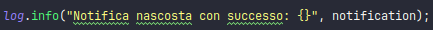
\includegraphics[scale=0.8]{img/log/logBack1.png}
  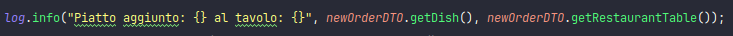
\includegraphics[scale=0.8]{img/log/logBack2.png}
  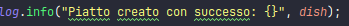
\includegraphics[scale=0.8]{img/log/logBack3.png}
  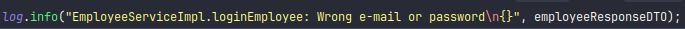
\includegraphics[scale=0.8]{img/log/logBack4.png}
  \caption{Log tramite SLF4J.}
\end{figure}
Mentre è stata usata la librerie \textbf{Log} di Android, per il log lato front-end.
\begin{figure}[H]
  \centering
  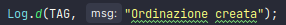
\includegraphics[scale=0.8]{img/log/logFront1.png}
  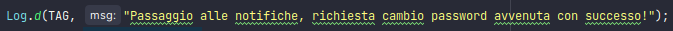
\includegraphics[scale=0.8]{img/log/logFront2.png}
  \caption{Log tramite \textit{Log}.}
\end{figure}